\documentclass[11pt, fleqn]{article}

\usepackage[usenames,dvipsnames,svgnames,table]{xcolor}
\usepackage{amsmath}
\usepackage{amsfonts}
\usepackage[margin=1in]{geometry} % To set the margin widths
\usepackage{graphicx}
\usepackage{listings}
\usepackage{multirow}
\usepackage{tabularx}
\usepackage{varioref}
\usepackage[noabbrev,capitalize]{cleveref}
\usepackage[group-separator={,}]{siunitx}
\usepackage{subcaption}
\usepackage{titlesec}
\usepackage{lscape}
\usepackage{bm}
\usepackage{chngpage}
\usepackage[titletoc,toc,title]{appendix}

\renewcommand\thesection{\arabic{section}}
\renewcommand\thesubsection{\thesection\alph{subsection}}

\lstset{
  frame=single,
  basicstyle=\ttfamily,% print whole listing small
  language=R,
  aboveskip=3mm,
  belowskip=3mm,
  showstringspaces=false,
  columns=flexible,
  numbers=none,
  commentstyle=\color{ForestGreen},
  stringstyle=\color{Maroon},
  breaklines=true,
  breakatwhitespace=true,
  tabsize=2,
  literate={<-}{{$\gets$}}1 {~}{{$\sim$}}1
}

\sisetup{output-exponent-marker=\textsc{e}}

\setlength{\parskip}{12pt} % Sets a blank line in between paragraphs
\setlength\parindent{0pt} % Sets the indent for each paragraph to zero

\begin{document}

\title{Homework \#4\\
Digital and Algorithmic Marketing (37304-01)}
\author{
Brian Chingono, Will Clark, Matthew DeLio, Jonathan Stevens (\textbf{Group \#8})\\
University of Chicago Booth School of Business}

\maketitle

\section{} (Jon) % Question 1

The number of possible message combinations that can be tested, or full factorial, is 1,024 message combinations. This number of combinations is a result of the number of factors that are being tested (7), and the number of levels for each factor.  The levels for the factors, in order from 1 to 7 are 4,4,2,2,2,4 and 2.  Thus, the number of combinations is equal to the product $4\times4\times2\times2\times2\times4\times2 = 1,024$.    

\section{} (Will) % Question 2

We estimate two logistic regression models, one for an open rate and one for a click rate:
\[ \log{\frac{p}{1-p}} = \bm{X}^{\prime} \bm{\beta} + \bm{\varepsilon} \]
where $p$ is the probability of a click or an open, $\bm{X}$ is the model matrix containing indicator variables for each factor/level combination, and $\bm{\beta}$ is the vector of estimated coefficients. We report the coefficients for the click and open models in \cref{tab:logit_results}, as well as the associated probabilities for each. Recall that we can express the coefficients as probabilities by:
\[ p = \frac{1}{1+\exp(-\beta)} \]
% latex table generated in R 3.2.5 by xtable 1.8-0 package
% Tue May  3 21:07:17 2016
\begin{table}[ht]
\centering
\caption{Logistic Regression Coefficients} 
\label{tab:logit_results}
\begin{tabular}{rrrrr}
  \hline
 & $\beta_j^{\text{open}}$ & $\exp(\beta_j^{\text{open}})$ & $\beta_j^{\text{click}}$ & $\exp(\beta_j^{\text{click}})$ \\ 
  \hline
\textsf{intro:L2} & 0.0127 & 1.01 & 0.00146 &    1 \\ 
  \textsf{intro:L3} & 0.0177 & 1.02 & 0.122 & 1.13 \\ 
  \textsf{intro:L4} & 0.00882 & 1.01 & -0.00526 & 0.995 \\ 
  \textsf{headline:L2} & 0.0106 & 1.01 & 0.0987 &  1.1 \\ 
  \textsf{headline:L3} & 0.00577 & 1.01 & 0.0802 & 1.08 \\ 
  \textsf{headline:L4} & 0.00837 & 1.01 & 0.0456 & 1.05 \\ 
  \textsf{main\_text:L2} & -0.00898 & 0.991 & -0.0116 & 0.989 \\ 
  \textsf{button:L2} & 0.000971 &    1 & -0.0101 & 0.99 \\ 
  \textsf{action:L2} & -0.0194 & 0.981 & 0.136 & 1.15 \\ 
  \textsf{purpose:L2} & 0.00639 & 1.01 & -0.0222 & 0.978 \\ 
  \textsf{purpose:L3} & -0.00481 & 0.995 & -0.0973 & 0.907 \\ 
  \textsf{purpose:L4} & -0.000423 &    1 & -0.0938 & 0.911 \\ 
  \textsf{symbol:L2} & 0.015 & 1.02 & -0.00475 & 0.995 \\ 
   \hline
\end{tabular}
\end{table}

We can make a few observations:
\begin{itemize}
\item The range of probabilities is higher in the click model (0.9 percent) than it is in the open model (5.8 percent). In general, the message variations have a larger marginal effect on click behavior (which is more valuable) than they do on open behavior.
\item The most powerful coefficient is the L2 level of the action type. 
\item Three of the top five strongest predictors of click rates are headlines (L2, L3, and L4). Choosing the proper headline makes a big difference in the final click rate.
\item Similarly, the three largest negative effects on click rate are different levels of the message purpose (L2, L3, and L4). So choosing the proper message purpose would be a way to minimize those who open but do not click a message.
\end{itemize}

\section{} % Question 3
We generated a full factorial of all 1,024 message combinations. Using this full factorial, we used our models to estimate open probabilities and click probabilities for each of the 1,024 message combinations. For comparison purposes, we also calculated the open and click probabilities for the control sample.

Our results are in \cref{fig:q3_hist} below. As shown in those histograms, there is a significant difference between the baseline click and open probabilities of the control message versus the estimated probabilities from our full factorial.

\begin{figure}[!htb]
  \centering
  \caption{Histogram of Predicted Probabilities vs. Control}
  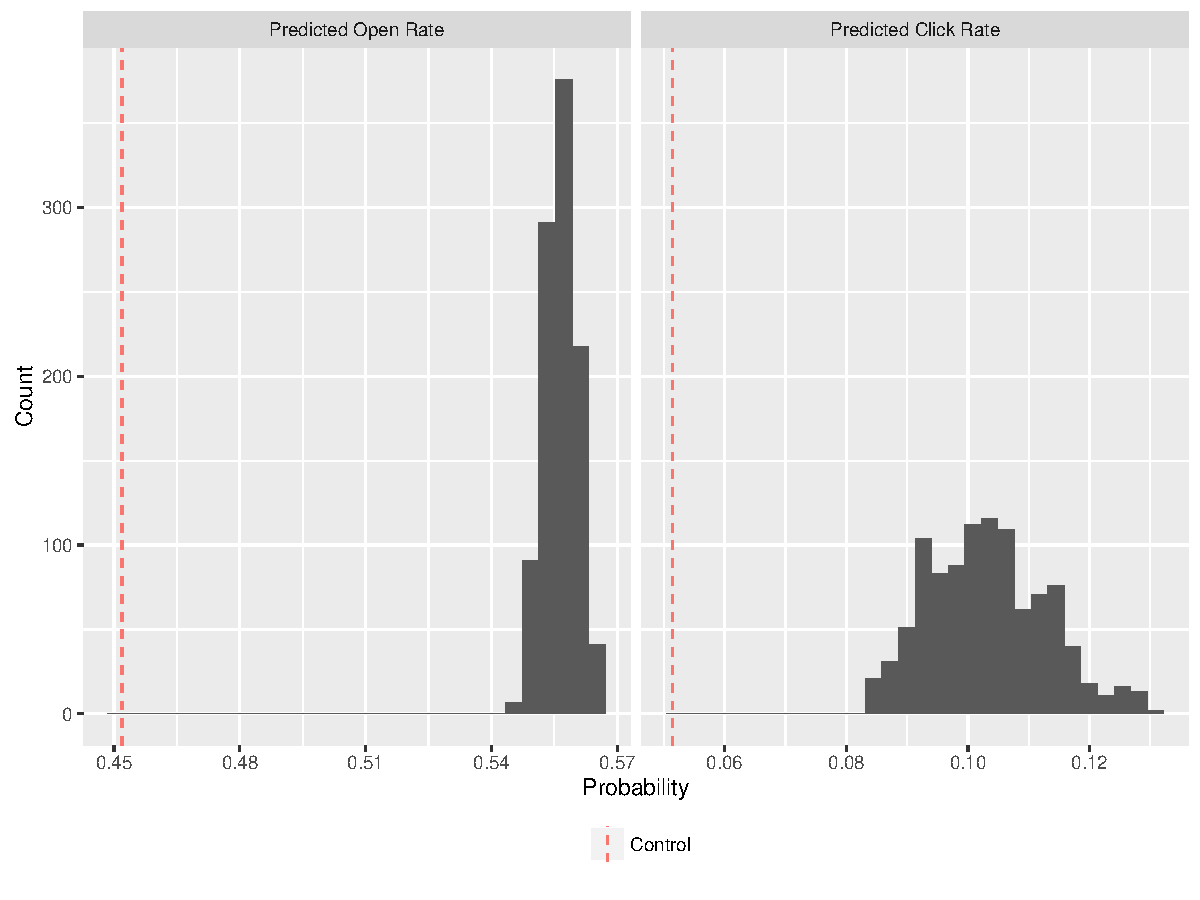
\includegraphics[scale=0.7]{q3_hist.pdf}
  \label{fig:q3_hist}
\end{figure}

In terms of message combinations with the highest estimated click and open rates, we found that 

\end{document}

% \input{.tex}

% \begin{figure}[!htb]
%   \centering
%   \caption{}
%   \begin{subfigure}[b]{0.49\textwidth}
%     \caption{}
%     \includegraphics[width=\textwidth]{.pdf}
%     \label{fig:}
%   \end{subfigure}
%   \hfill
%   \begin{subfigure}[b]{0.49\textwidth}
%     \caption{}
%     \includegraphics[width=\textwidth]{.pdf}
%     \label{fig:}
%   \end{subfigure}
% \end{figure}

% \begin{figure}[!htb]
%   \centering
%   \caption{}
%   \includegraphics[scale=.5]{.pdf}
%   \label{fig:}
% \end{figure}